\documentclass[border=-10mm]{standalone}
\usepackage{pgfplots}
\usepackage{tikz}
\usepackage{xcolor}

\begin{document}

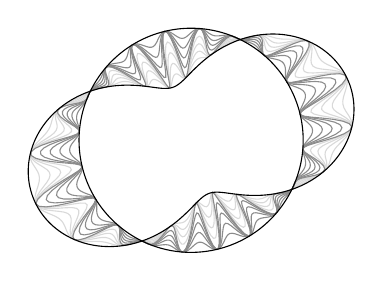
\begin{tikzpicture}
  \begin{axis}[axis lines=none, axis equal,
    xmin=-2,xmax=2,
    ymin=-2,ymax=2,
    samples=300
    ]

    % Path 2
    \foreach \t in {1,...,4}
    \addplot[gray!30, domain=0:360]
    ({
      cos(x)*( \t /5*(1+sin((x+45)*20))/2) + (1+sin((x +
      26)*2)/2*1)*cos(x)*
      (1-\t /5*(1+sin((x+45)*20))/2)
    },
    {
      sin(x)*( \t /5*(1+sin((x+45)*20))/2) + (1+sin((x +26)*2)/2*1)*sin(x)*
      (1- \t /5*(1+sin((x+45)*20))/2)
    });

    % \addplot[gray!30, domain=0:360]
    % ({
    %   cos(x)*(1- 5 /5*(1+sin(x*20))/2) + (1+sin((x +
    %   26)*2)/2*1)*cos(x)*
    %   (5 /5*(1+sin(x*20))/2)
    % },
    % {
    %   sin(x)*(1- 5 /5*(1+sin(x*20))/2) + (1+sin((x +26)*2)/2*1)*sin(x)*
    %   (5 /5*(1+sin(x*20))/2)
    % });

    %   Path 1
    \foreach \t in {1,...,4}
    \addplot[gray!90,   domain=0:360]
    ({
      cos(x)*(1- \t /5*(1+sin(x*20))/2) + (1+sin((x +
      26)*2)/2*1)*cos(x)*
      (\t /5*(1+sin(x*20))/2)
    },
    {
      sin(x)*(1- \t /5*(1+sin(x*20))/2) + (1+sin((x +26)*2)/2*1)*sin(x)*
      (\t /5*(1+sin(x*20))/2)
    });

    \addplot[gray!90,   domain=0:360]
    ({
      cos(x)*(1- 5 /5*(1+sin(x*20))/2) + (1+sin((x +
      26)*2)/2*1)*cos(x)*
      (5 /5*(1+sin(x*20))/2)
    },
    {
      sin(x)*(1- 5 /5*(1+sin(x*20))/2) + (1+sin((x +26)*2)/2*1)*sin(x)*
      (5 /5*(1+sin(x*20))/2)
    });

    % q0 and q1
    \addplot[domain=0:360]
    ({cos(x)},{sin(x)});

    \addplot[domain=0:36]
    ({(1+sin((x *10 + 26)*2)/2*1)*cos(x *10)},{(1+sin((x *10 +
      26)*2)/2*1)*sin(x *10)});
  \end{axis}
\end{tikzpicture}

\end{document}


